\documentclass[a4paper]{article}

\usepackage{cite} % cite multiple reference
\usepackage{graphicx}
\usepackage{array} % change the height of rows in a tabular
\usepackage{multirow,makecell} % allows multiple rows in tabular
\usepackage{tabularx} % allow fixed height tabular
\usepackage{subfigure}
\usepackage{titlesec} % title format
\usepackage{amsmath}
\usepackage{amssymb}
\usepackage{tabularx}
\usepackage{makecell}
\usepackage{geometry}
\usepackage{float}
\usepackage{setspace} % set the space between lines 
\usepackage{siunitx}
\usepackage{mdwlist}
\usepackage{tabu}
\usepackage{enumerate}
\usepackage{circuitikz}
\usepackage{tikz}
\usetikzlibrary{arrows,positioning,shapes,backgrounds,fit} 

\geometry{top=1.54cm,bottom=2.54cm,left=2.5cm,right=2.5cm}

\begin{document}
\begin{center}
\bf\Large
ME  180  Digital Control/Dynamic System\par
Department of Mechanical Engineering\par
Tufts University Fall 2019\par
Problem Set \#1\par
\end{center}
\begin{table}[H]
\begin{center}
\begin{tabular*}{\textwidth}{@{\extracolsep{\fill}}lcr}
Name: Shang Wang &Student ID: 1277417 &E-mail: shang.wang@tufts.edu\\
\hline
\end{tabular*}
\end{center}
\end{table}

\section{Problem P2.9(b)}
{\par\noindent \bf\large  Description   \par}
For each of the following transfer functions, write the
corresponding differential equation. 
\par Section (b) 
$$\frac{X(s)}{F(s)} = \frac{15}{(s+10)(s+11)}$$
{\par\noindent\bf\large Solution \par}
Rewrite the transfer function $G(s) = X(s)/F(s)$ as $F(s) = [1/G(s)] X(s)$, which is:
$$
F(s) = \frac{1}{15} (s^2 + 21s + 110) X(s) 
$$
Then:
$$
F(s) = \frac{1}{15} s^2X(s) + \frac{7}{5}sX(s) + \frac{22}{3}X(s)
$$
Take the inver laplace transform on both sides and ignore the initial value(set to zero):
$$
f(t) = \frac{1}{15} \frac{d^2}{dt^2}x(t) + \frac{7}{5}\frac{d}{dt}x(t) + \frac{22}{3}x(t)
$$

\section{Problem P2.19(a)}
{\par\noindent \bf\large  Description   \par}
Find the transfer function,	$G(s) = V_o(s)/V_i(s)$, for each network shown in Figure. Solve the problem using mesh analysis. 
\par Section (a) Circuit 
\begin{figure}[H]
\centering
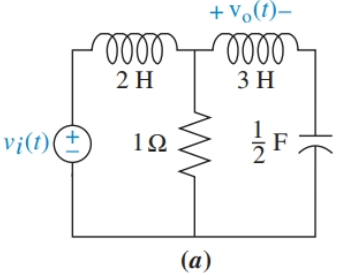
\includegraphics[width=0.4\textwidth]{pic/ch2_19a.png}
\caption{P2.19(a)} 
\end{figure}

{\par\noindent\bf\large Solution \par}
The mesh equations are:
$$
\begin{aligned}
    &I_1(s)(sL_1 + R) &&-I_2(s)R &&= V_{in}\\
    -&I_1(s)R &&+I_2(s)(R + sL_2 + \frac{1}{sC}) &&= 0\\
\end{aligned}
$$
\begin{figure}[H]
\centering
    \begin{circuitikz}[scale=1.2]
    \ctikzset{resistors/scale=0.8, % smaller R
    capacitors/scale=0.7, % even smaller C
    sources/scale=0.8} 
    \draw (0,0)  
    to[vsource, v= $v_{in}$](0,3)
    to[L=$L_1$, i>=$i_1$] (2,3)
    to[short, -*] (2,3)
    to[R=$R$, i>_=$i_3$] (2,0) -- (0,0);
    \draw (2,3) 
    to[L=$L_2$, a=$v_{out}$, i>=$i_2$] (4,3)
    to[C=$C$, i>] (4,0) -- (0,0);
\end{circuitikz}
\end{figure}
Then solve $I_2(s)$ from the equation:
$$
\begin{aligned}
 I_2(s) = 
    \begin{bmatrix}
    sL_1+R &V_{in}\\
    -R &0\\
    \end{bmatrix}
    \Big /
    \begin{bmatrix}
    sL_1+R &-R\\
    -R &R + sL_2 + \frac{1}{sC} 
    \end{bmatrix}
    = \frac{sRC}{s^3(L_1L_2C) + s^2(L_1+L_2)RC + sL_1 + R}V_{in}(s)
\end{aligned}
$$
Then we can get:
$$
V_{out}(s) = I_2(s)(sL_2) = \frac{s^2L_2RC}{s^3(L_1L_2C) + s^2(L_1+L_2)RC + sL_1 + R}V_{in}(s)
$$
Substitute the variables with the value above, then the transfer function is:
$$
T(s) = \frac{V_{out}(s)}{V_{in}(s)} = \frac{3s^2}{6s^3+5s^2+4s+2}
$$

\section{Problem P2.25}
{\par\noindent \bf\large  Description   \par}
Find the transfer function, $G(s) = X_2(s)/F(s)$, for the translational mechanical network shown in Figure P2.25.
\begin{figure}[H]
\centering
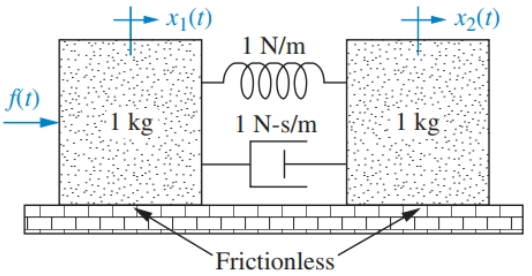
\includegraphics[width=0.4\textwidth]{pic/ch2_25.png}
\caption{P2.25} 
\end{figure}

{\par\noindent\bf\large Solution \par}
According to the text, we could obtain the dynamics of this mechanical system:
$$
\begin{aligned}
    &X_1(s)(m_1s^2 + \zeta s + k) &&-X_2(s)(\zeta s + k) &&= F(s)\\
    -&X_1(s)(\zeta s + k) &&+X_2(s)(m_2s^2 + \zeta s + k) &&= 0\\ 
\end{aligned}
$$
Substitute with the value above
$$
\begin{aligned}
    &X_1(s)(s^2 +  s + 1) &&-X_2(s)( s + 1) &&= F(s)\\
    -&X_1(s)( s + 1) &&+X_2(s)(s^2 +  s + 1) &&= 0\\ 
\end{aligned}
$$
which could be solved by Cramer's Rule,
$$
X_2(s) = 
\begin{bmatrix}
    s^2+s+1 &F(s)\\
    -(s+1)  &0\\
\end{bmatrix}\Big/
\begin{bmatrix}
    s^2+s+1 &s+1\\
    -(s+1)  &s^2+s+1\\
\end{bmatrix}
= \frac{s+1}{(s^2+2s+2)s^2}F(s)
$$
Thus the transfer function is:
$$
\frac{X(s)}{F(s)} = \frac{s+1}{(s^2+2s+2)s^2}
$$
{\bf Bonus:} the equavalant circuit dynamics should be like:
$$
\begin{aligned}
    &\frac{1}{s}I_1(s)(L_1s^2 + R s + \frac{1}{C}) &&-\frac{1}{s}I_2(s)(R s + \frac{1}{C}) &&= V_{in}(s)\\
    -&\frac{1}{s}I_1(s)(R s + \frac{1}{C}) &&+\frac{1}{s}I_2(s)(L_2s^2 + R s + \frac{1}{C}) &&= 0\\ 
\end{aligned}
$$
Thus the schematic of the equavaent circuit is: 
\begin{figure}[H]
\centering
    \begin{circuitikz}[scale=1.0]
    \ctikzset{resistors/scale=0.8, % smaller R
    capacitors/scale=0.7, % even smaller C
    sources/scale=0.8} 
    \draw (0,3) 
    to[short, o-, l=$v_{in}$] (0,3)
    to[L=$L_1\sim m_1$, i_>=$i_1$] (2,3)
    to[short, -*] (2,3)
    to[R=$R\sim \zeta $, i_>=$i_3$] (2,1)
    to[C, l=$C\sim \frac{1}{k}$, i>] (2,0.5) -- (2,0)
       node[ground]{}(2,-0.5);
    \draw (2,3) 
    to[L=$L_2\sim m_2$, i>_=$i_2$] (4,3) -- (4,0) 
    to[short, -*] (2,0);
\end{circuitikz}
\end{figure}
while the input should be $V_{in}(s)$, the output should be $\frac{1}{s}I_2(s)$. To obtain the output, consider using a AMP intergrator:
\begin{figure}[H]
\centering
    \begin{circuitikz}[scale=1.0]
    \ctikzset{resistors/scale=1, % smaller R
    capacitors/scale=1, % even smaller C
    inductors/scale=1.3} 
 
    \draw (5.5,3.5)
    node[op amp] (opamp) {};
    \draw (opamp.out) to[short, l_=$sL_2i_2$] ++(0.5,0) coordinate(tmp2);
    \draw (opamp.-) to [short] ++(-0.2,0) to[short]++ (0,1) coordinate(tmp) to[short] (tmp -| tmp2) to[short,-*] (tmp2);
    % \draw (opamp.-) to [short, -*] ++(-0.2,0) node[ground] {};
    \draw (opamp.+) to[short] ++ (-0.5,0) 
    to[short] ++(-1,0)
    to[short, -*] ++ (0,0) coordinate(tmp3)
    to[R, l_=$R\sim \zeta $, i_>=$i_3$] ++ (0,-2)
    to[C, l_=$C\sim \frac{1}{k}$, i>] ++ (0,-1) 
       node[ground]{} ++ (0,-0.1);
    \draw (tmp3) 
    to[L, l_=$L_1\sim m_1$, mirror, i<=$i_1$] ++ (-2,0)
    to[short, -o, l=$v_{in}$] ++ (-0.0,0);
    \draw (opamp.+) 
    to [short, -*] ++ (-0.5, 0)
    to[L, l=$L_2\sim m_2$, i>_=$i_2$] ++(0,-3.0)
    to [short, -*] ++ (-1, 0);
    
    \draw (10.5,3)
    node[op amp] (opamp2) {};
    \draw (opamp2.out) to[short] ++(0.5,0) coordinate(tmp2) node[right] {$v_{out}=-L_2i_2/(sLC)$};
     
    \draw (opamp2.-) to [short, -*] ++(-0.2,0) to[short]++ (0,1) coordinate(tmp) to[C=$C$] (tmp -| tmp2) to[short,-o] (tmp2);
    % \draw (opamp.-) to [short, -*] ++(-0.2,0) node[ground] {};
    \draw (opamp.out) to [short] ++ (0.5,0)
    to [L= $L$] (opamp2.-);
    \draw (opamp2.+) to [short] ++(-0,-0.5) node[ground] {};

\end{circuitikz}
\end{figure}
Then pick $LC = L_2$, we can obtain the $I(s)/s$ presented in the form of voltage. 

\section{Problem P2.35}
{\par\noindent \bf\large  Description   \par}
 For the rotational mechanical system with gears shown in Figure P2.20,find the transfer function, $G(s) = \theta_3(s)/T(s)$. The gears have inertia and bearing friction as shown. [ {\bf notes of instructor: }Do not solve the TF.  Instead, determine apparent inertia at $\theta_3$ ]

 {\par\noindent\bf\large Solution \par}
The transfer function of the this gear system should have a form of:
$$
(\gamma_1 \gamma_2) T(s) = (J_{eq}s^2 + D_{eq}s + K_{eq})\Theta_3(s)
$$
where $\gamma_1 =\frac{N_1}{N_2} $, $\gamma_2 = \frac{N_3}{N_4}$, are the gear ratio. And $J_{eq}$, $D_{eq}$, $K_{eq}$ represent the equavalant impedance. Thus,
$$
\begin{aligned}
J_{eq} &= J_5 + J_4 + \gamma_2^2[J_3 + J_2 + \gamma_1^2(J_1)]\\
       &= J_5 + J_4 + \gamma_2^2(J_3 + J_2) + \gamma_2^2\gamma_1^2J_1\\
       &=J_5 + J_4 + \Big (\frac{N_3}{N_4}\Big )^2(J_3 + J_2) + \Big (\frac{N_3}{N_4}\Big )^2\Big (\frac{N_1}{N_2}\Big )^2J_1\\  
\end{aligned}
$$

\section{Problem P2.54}
{\par\noindent \bf\large  Description   \par}
Consider the differential equation:
$$
\frac{d^3 x}{dt^3} + 10 \frac{d^2 x}{dt} + 20\frac{dx}{dt} + 15x = f(x)
$$
where is the input and is a function of the output, $x$.If $f(x) = 3e^{-5x}$, linearize the differential equation for $x$ near 0.[ {\bf notes instructor:} linearize at $x=1$ instead of $x=0$ ]
{\par\noindent\bf\large Solution \par}
the component $f(x) = 3e^{-5x}$ is a nonlinear component in terms of $x(t)$, thus
\begin{enumerate}
    \item determine the operating point, which corresponds to $x_0 = 1$: 
    $$ f_0 = f(1) = 3e^{-5} $$
    \item determine the slop in terms of $x$ at the operating point :
    $$ m = \frac{\partial f}{\partial x}\Big|_{x = x_0} = (-15)e^{-5x}\Big|_{x = x_0} = -15e^{-5}  $$
    \item change of variables, using the local linearized function $\delta f = f_0 + m\delta x$ to approximate the original nonlinear function $f$,
    $$ \delta f = 3e^{-5} +  (-15)e^{-5}\delta x, \ \  \delta x = x - x_0 $$
\end{enumerate}
The local linearized differential equation in terms of $\delta x$ at operating point $x_0 = 1$ is: 
$$
\frac{d^3}{dt^3}\delta x + 10 \frac{d^2}{dt}\delta x + 20\frac{d}{dt}\delta x + 15\delta x =  3e^{-5} +  (-15)e^{-5}\delta x
$$

\section{Problem P5.13}
{\par\noindent \bf\large  Description   \par}
For the system shown in Figure P5.13, find the poles of the closed-loop transfer function, $T(s)=C(s)/R(s)$. [ {\bf notes of instructor: }obtain the transfer function  ] 
\begin{figure}[H]
\centering
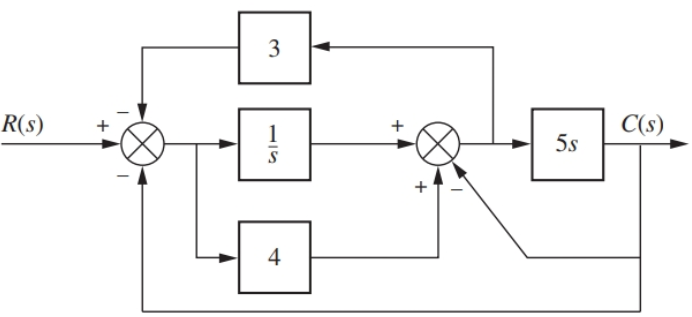
\includegraphics[width=0.6\textwidth]{pic/ch5_13.png}
\caption{P5.13} 
\end{figure}

{\par\noindent\bf\large Solution \par}
First, get the input $X(s)$ of the $1/s$ block:
$$ 
X(s) = R(s) - \frac{3C(s)}{5s} - C(s)
$$
Then calculate the equation of the second nodes:
$$ 
\frac{C(s)}{5s} = (\frac{1}{s} + 4)X(s) - C(s)
$$
Substitute the $X(s)$ in the second equation by the first equation:
$$ 
\frac{C(s)}{5s} = \Big(\frac{1}{s} + 4\Big)\Big(R(s) - \frac{3C(s)}{5s} - C(s)\Big) - C(s)
$$
Then
$$
(25s^2 + 22s + 3) C(s) = (20s^2 + 5s)R(s)
$$
$$
G(s) = \frac{C(s)}{R(s)} = \frac{20s^2 + 5s}{25s^2 + 22s + 3}
$$




\end{document}